% =============================================================================
%
% =============================================================================
\documentclass[11pt,a4paper,fleqn]{scrartcl}
\usepackage{et-labor}
%\usepackage{graphicx}

\Jahrgang{4AHET}
\Gruppe{4}
\Nummer{4}
\Uebung{Sternpunktverschiebung}
\Lehrer{Prof. Berger}
\Uebungsdatum{14.09.2022}
\Abgabedatum{21.09.2022}
\Schueler{HIEGESBERGER Raphael\\ NUSSBAUM Daniel\\TRAXLER Marlene}
\Schriftfuehrer{TRAXLER Marlene}

\begin{document}
	\indextrue   % aktivieren, wenn Inhaltsverzeichnis auf die Titelseite soll
\Titelseite
\ifindex\else\tableofcontents\newpage\fi

% =====================================================
\section{Sym. Stern mit N}
% =====================================================
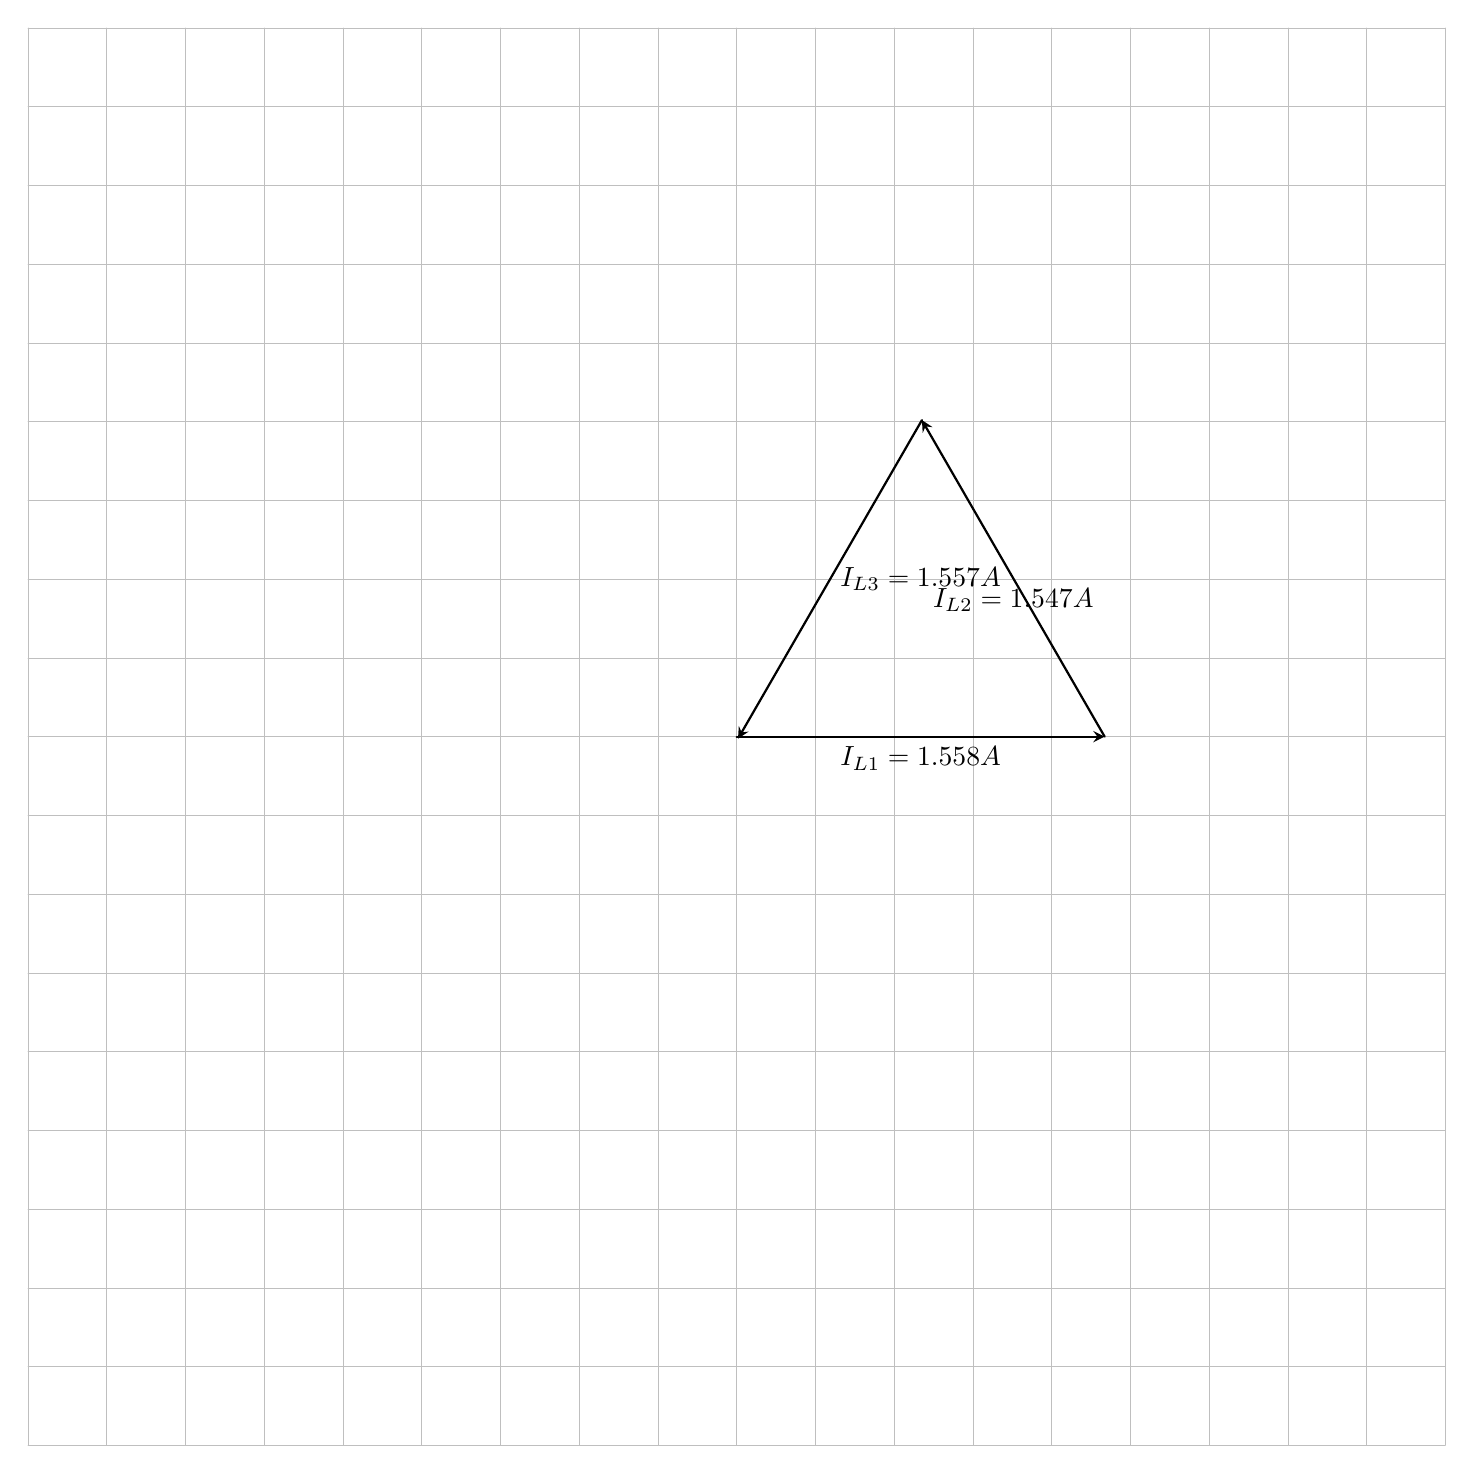
\begin{tikzpicture}[
	>=stealth,
	thick,
	line cap=round,
	line join=round
	]
	\draw[help lines,lightgray] (-9,-9) grid (9,9);
	\begin{scope}[->]
		\draw (0.0,0.0) -- (4.674,0.0) node[midway,below] {$I_{L1}=1.558A$};
		\draw (4.674,0.0) -- (2.3535000000000013,4.01922389896358) node[midway,below] {$I_{L2}=1.547A$};
		\draw (2.3535000000000013,4.01922389896358) -- (0.01800000000000246,-0.02598076211353284) node[midway,right] {$I_{L3}=1.557A$}; 
	\end{scope}
\end{tikzpicture}


% =====================================================
\section{Sym. Stern mit N}
% =====================================================
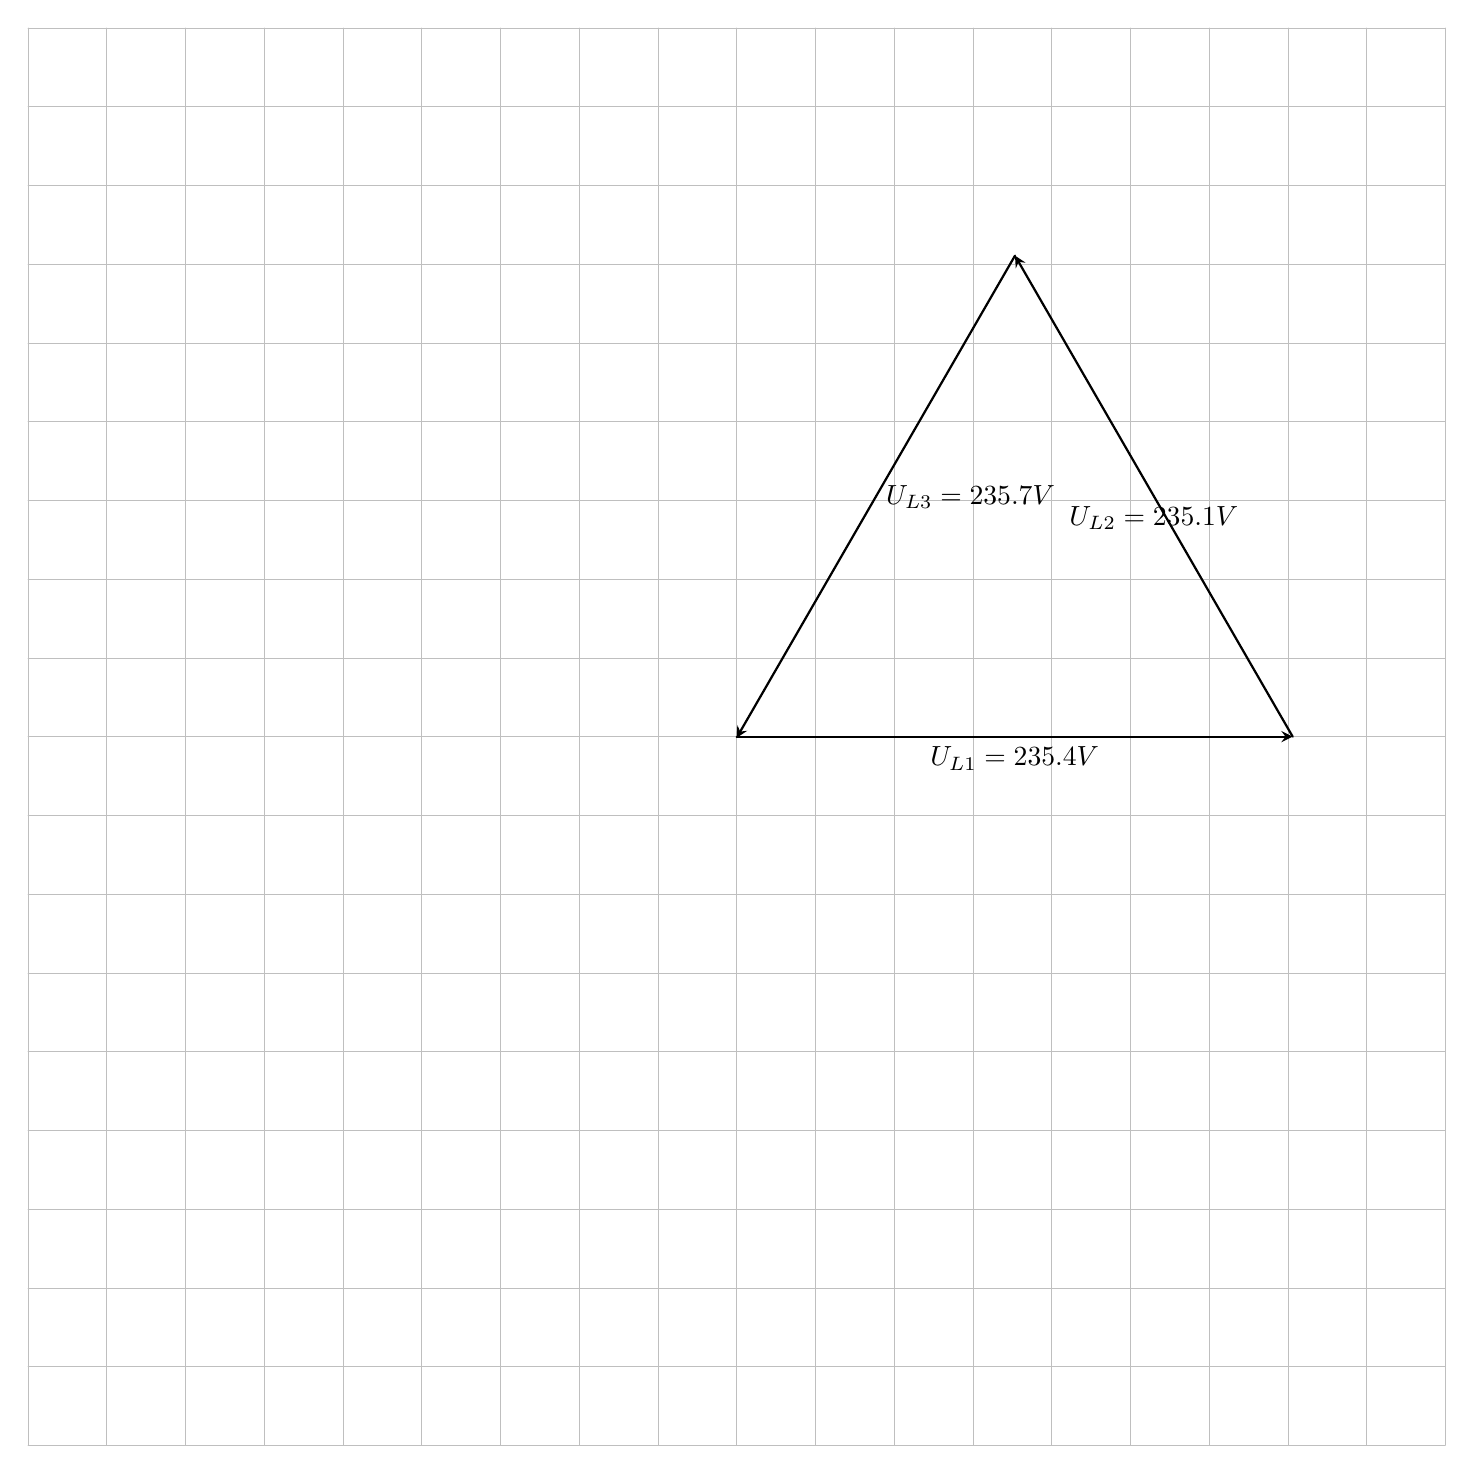
\begin{tikzpicture}[
	>=stealth,
	thick,
	line cap=round,
	line join=round
	]
	\draw[help lines,lightgray] (-9,-9) grid (9,9);
	\begin{scope}[->]
		\draw (0.0,0.0) -- (7.062,0.0) node[midway,below] {$U_{L1}=235.4V$};
		\draw (7.062,0.0) -- (3.535500000000002,6.1080771728916465) node[midway,below] {$U_{L2}=235.1V$};
		\draw (3.535500000000002,6.1080771728916465) -- (3.9968028886505635E-15,-0.015588457268119527) node[midway,right] {$U_{L3}=235.7V$}; 
	\end{scope}
\end{tikzpicture}


% =====================================================
\section{Sym. Stern ohne N}
% =====================================================
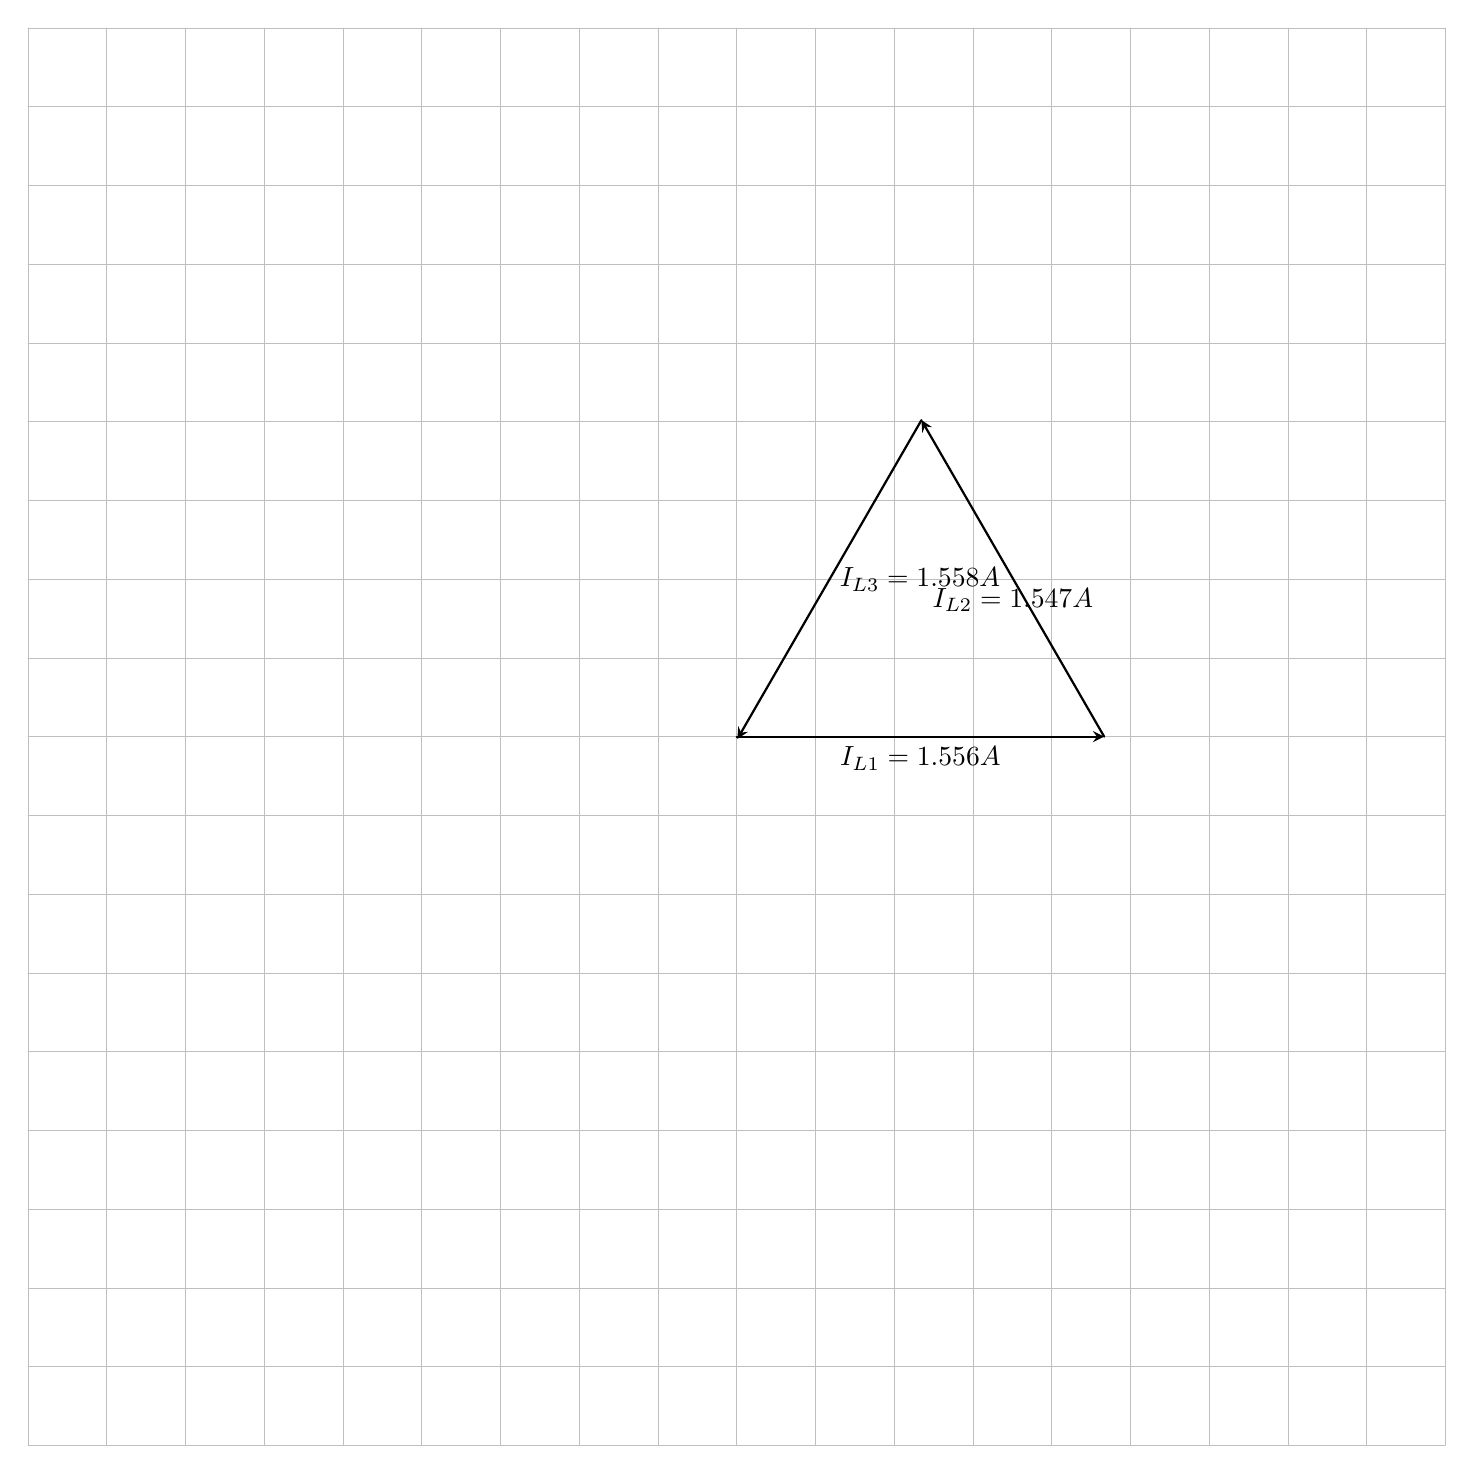
\begin{tikzpicture}[
	>=stealth,
	thick,
	line cap=round,
	line join=round
	]
	\draw[help lines,lightgray] (-9,-9) grid (9,9);
	\begin{scope}[->]
		\draw (0.0,0.0) -- (4.668,0.0) node[midway,below] {$I_{L1}=1.556A$};
		\draw (4.668,0.0) -- (2.347500000000001,4.01922389896358) node[midway,below] {$I_{L2}=1.547A$};
		\draw (2.347500000000001,4.01922389896358) -- (0.01050000000000173,-0.02857883832488639) node[midway,right] {$I_{L3}=1.558A$}; 
	\end{scope}
\end{tikzpicture}


% =====================================================
\section{Sym. Stern ohne N}
% =====================================================
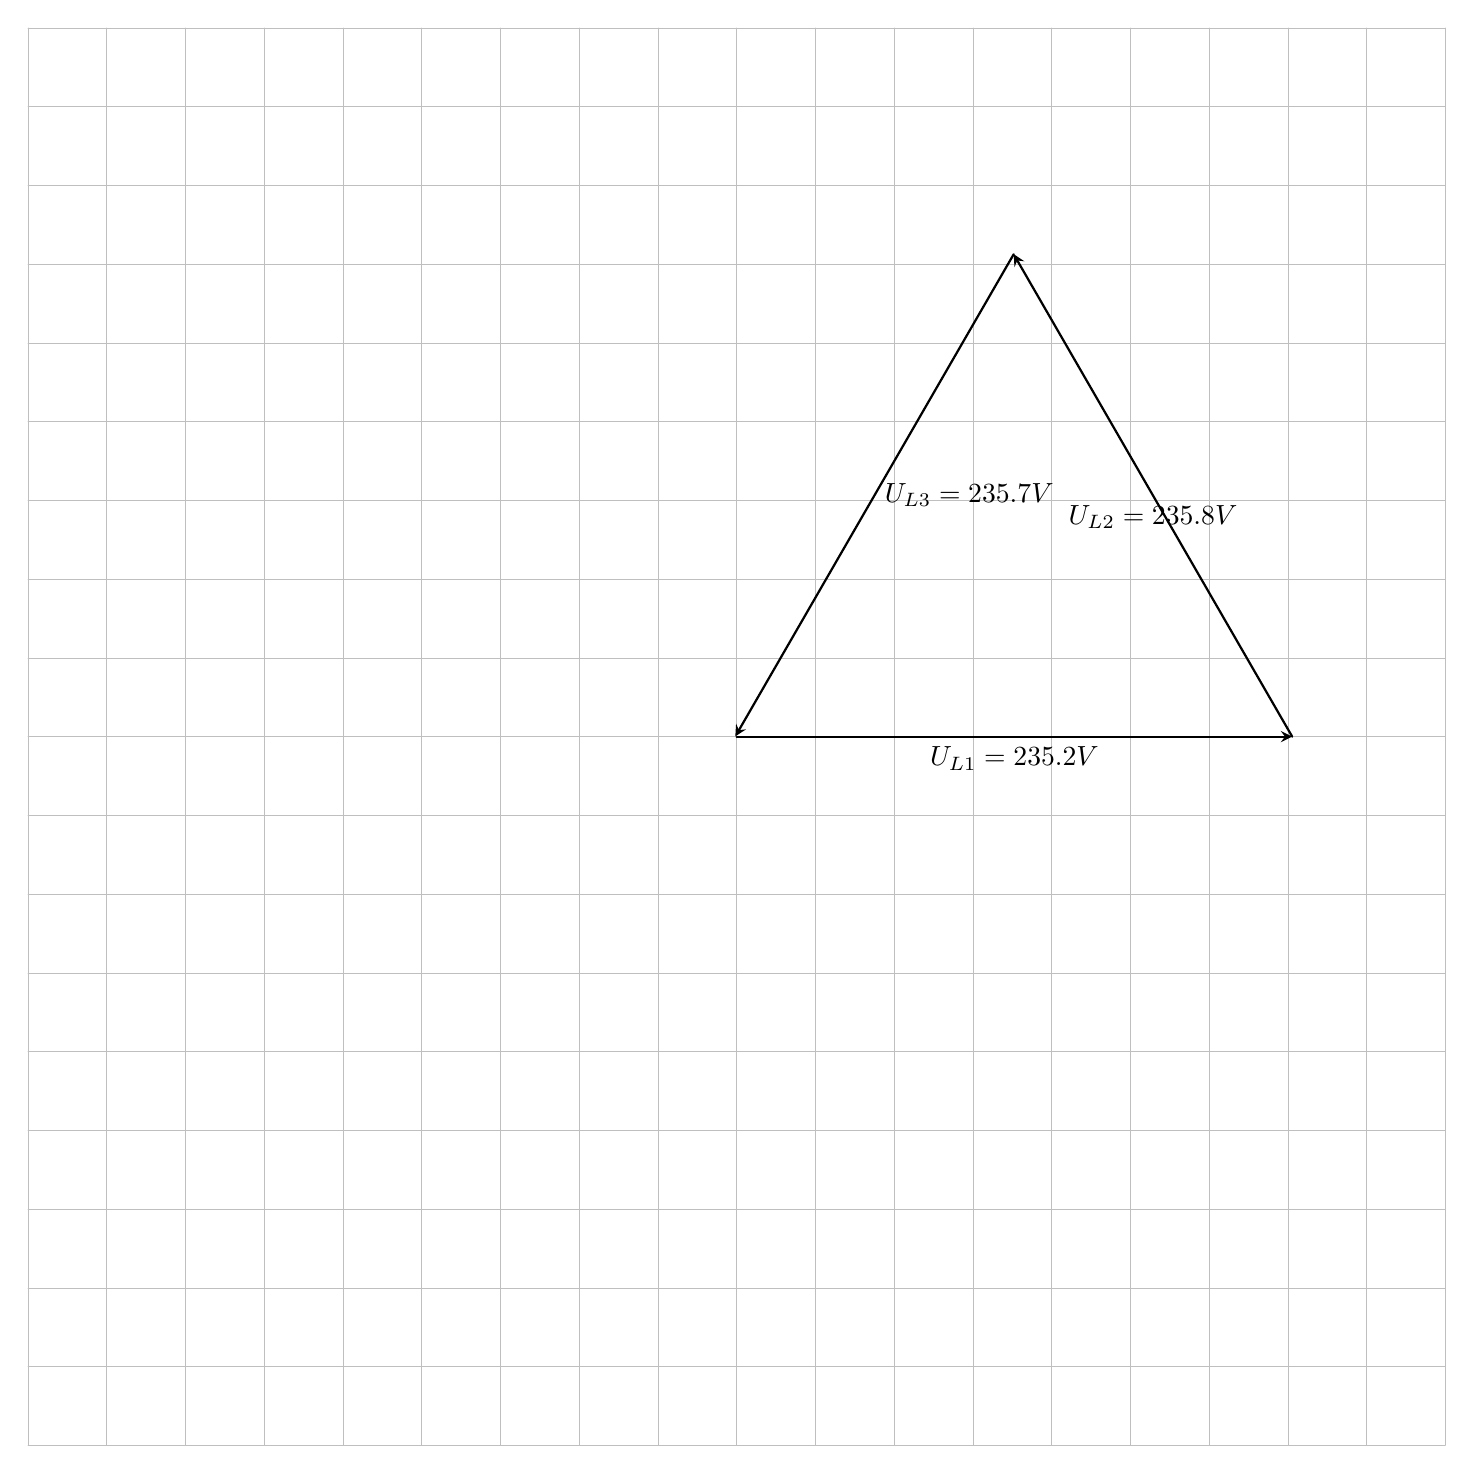
\begin{tikzpicture}[
	>=stealth,
	thick,
	line cap=round,
	line join=round
	]
	\draw[help lines,lightgray] (-9,-9) grid (9,9);
	\begin{scope}[->]
		\draw (0.0,0.0) -- (7.055999999999999,0.0) node[midway,below] {$U_{L1}=235.2V$};
		\draw (7.055999999999999,0.0) -- (3.519000000000001,6.12626370637112) node[midway,below] {$U_{L2}=235.8V$};
		\draw (3.519000000000001,6.12626370637112) -- (-0.016499999999997073,0.0025980762113535505) node[midway,right] {$U_{L3}=235.7V$}; 
	\end{scope}
\end{tikzpicture}


% =====================================================
\section{Unsym. Stern mit N}
% =====================================================
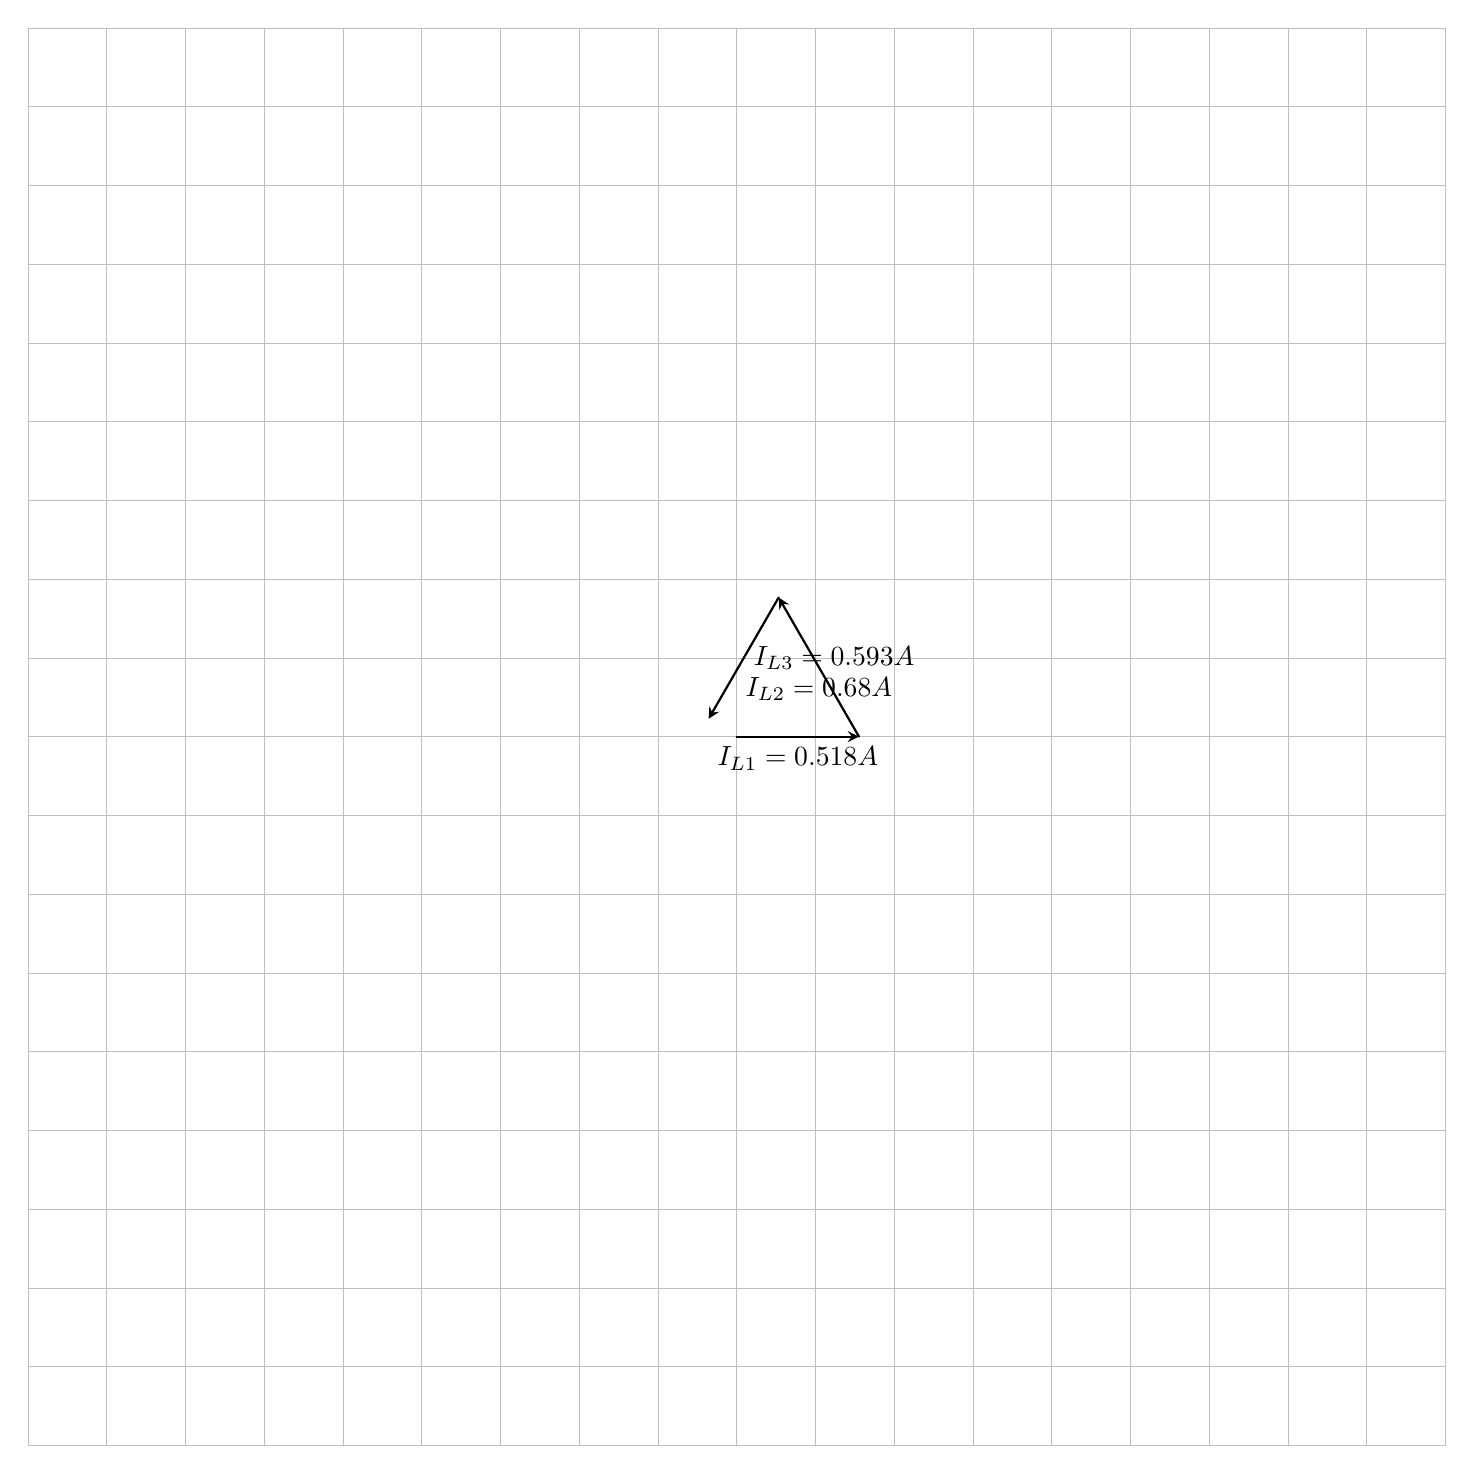
\begin{tikzpicture}[
	>=stealth,
	thick,
	line cap=round,
	line join=round
	]
	\draw[help lines,lightgray] (-9,-9) grid (9,9);
	\begin{scope}[->]
		\draw (0.0,0.0) -- (1.554,0.0) node[midway,below] {$I_{L1}=0.518A$};
		\draw (1.554,0.0) -- (0.5340000000000005,1.766691823720255) node[midway,below] {$I_{L2}=0.68A$};
		\draw (0.5340000000000005,1.766691823720255) -- (-0.35549999999999904,0.22603263038773846) node[midway,right] {$I_{L3}=0.593A$}; 
	\end{scope}
\end{tikzpicture}


% =====================================================
\section{Unsym. Stern mit N}
% =====================================================
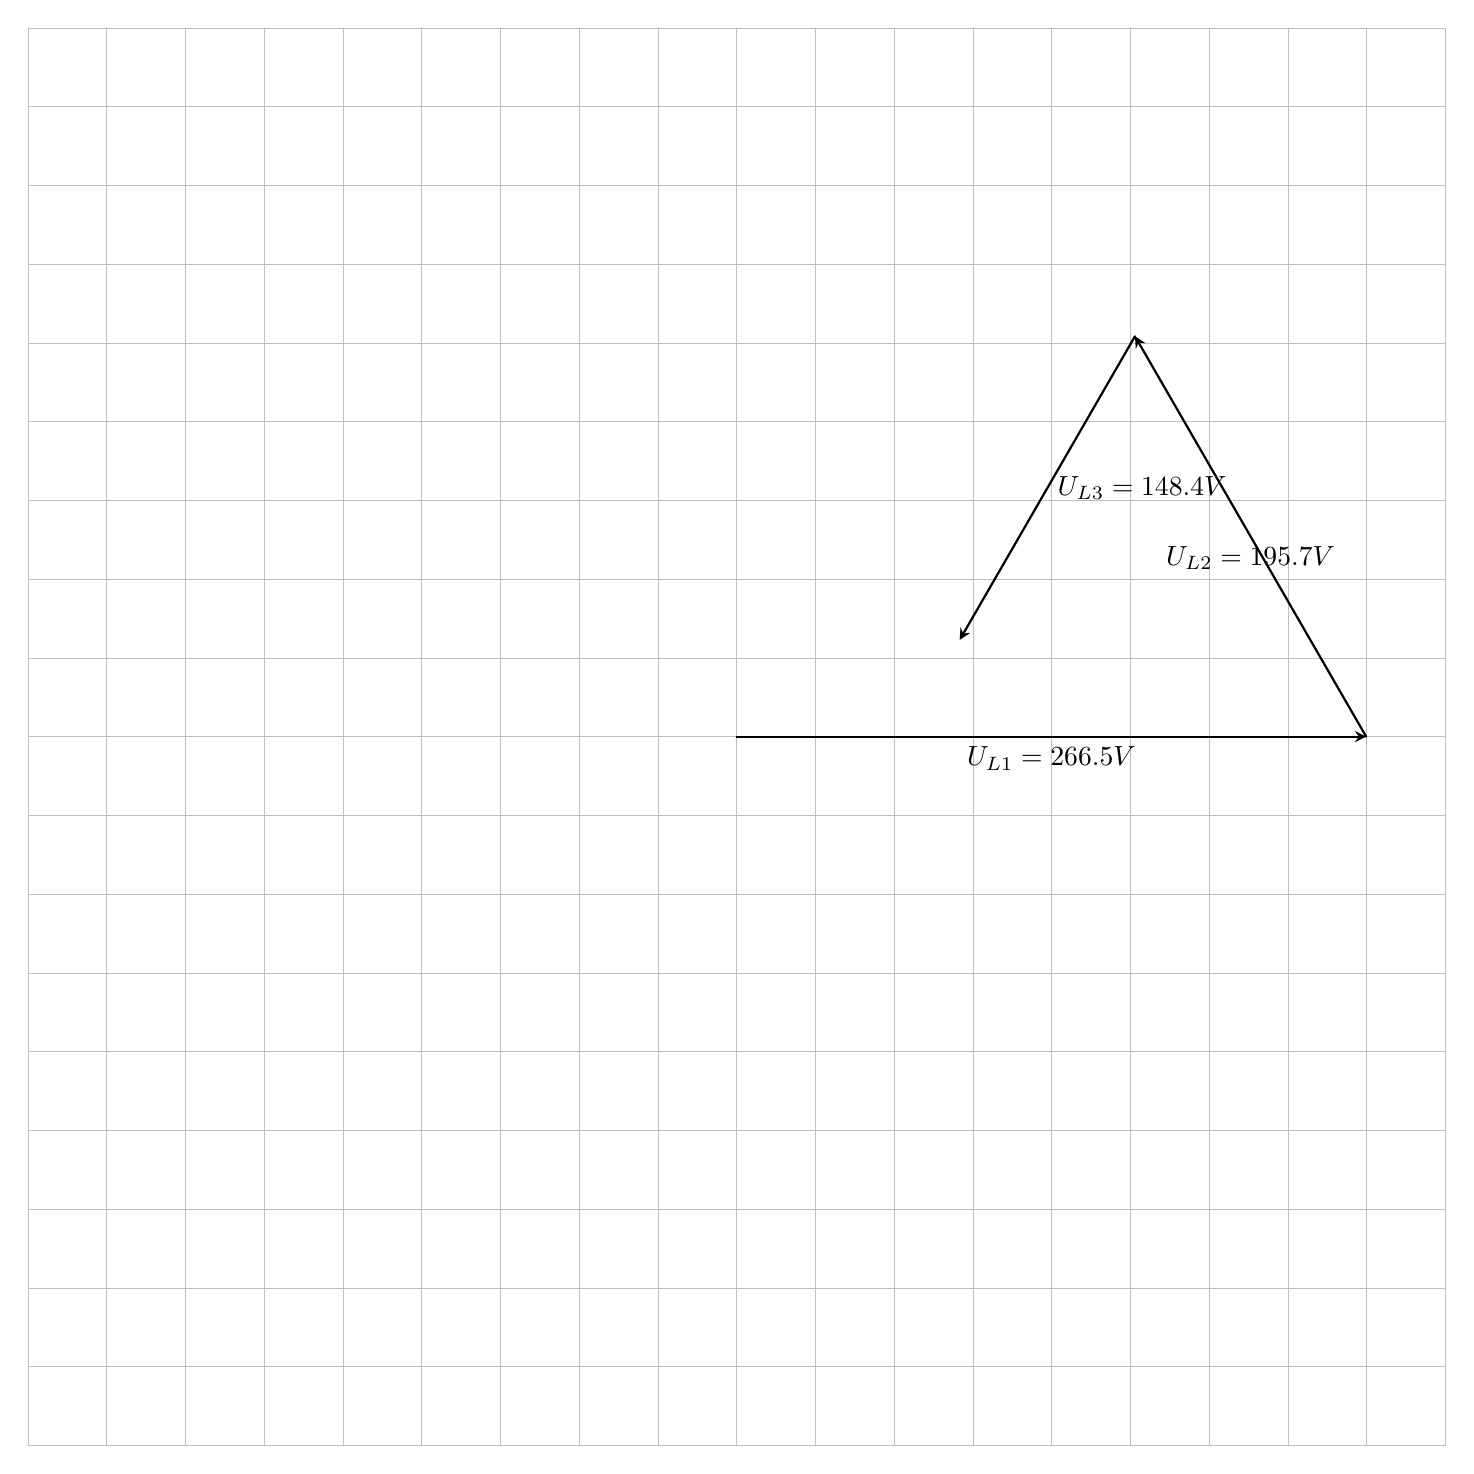
\begin{tikzpicture}[
	>=stealth,
	thick,
	line cap=round,
	line join=round
	]
	\draw[help lines,lightgray] (-9,-9) grid (9,9);
	\begin{scope}[->]
		\draw (0.0,0.0) -- (7.995,0.0) node[midway,below] {$U_{L1}=266.5V$};
		\draw (7.995,0.0) -- (5.059500000000002,5.084435145618439) node[midway,below] {$U_{L2}=195.7V$};
		\draw (5.059500000000002,5.084435145618439) -- (2.8335000000000026,1.228890047970118) node[midway,right] {$U_{L3}=148.4V$}; 
	\end{scope}
\end{tikzpicture}


% =====================================================
\section{Sym. Dreieck}
% =====================================================
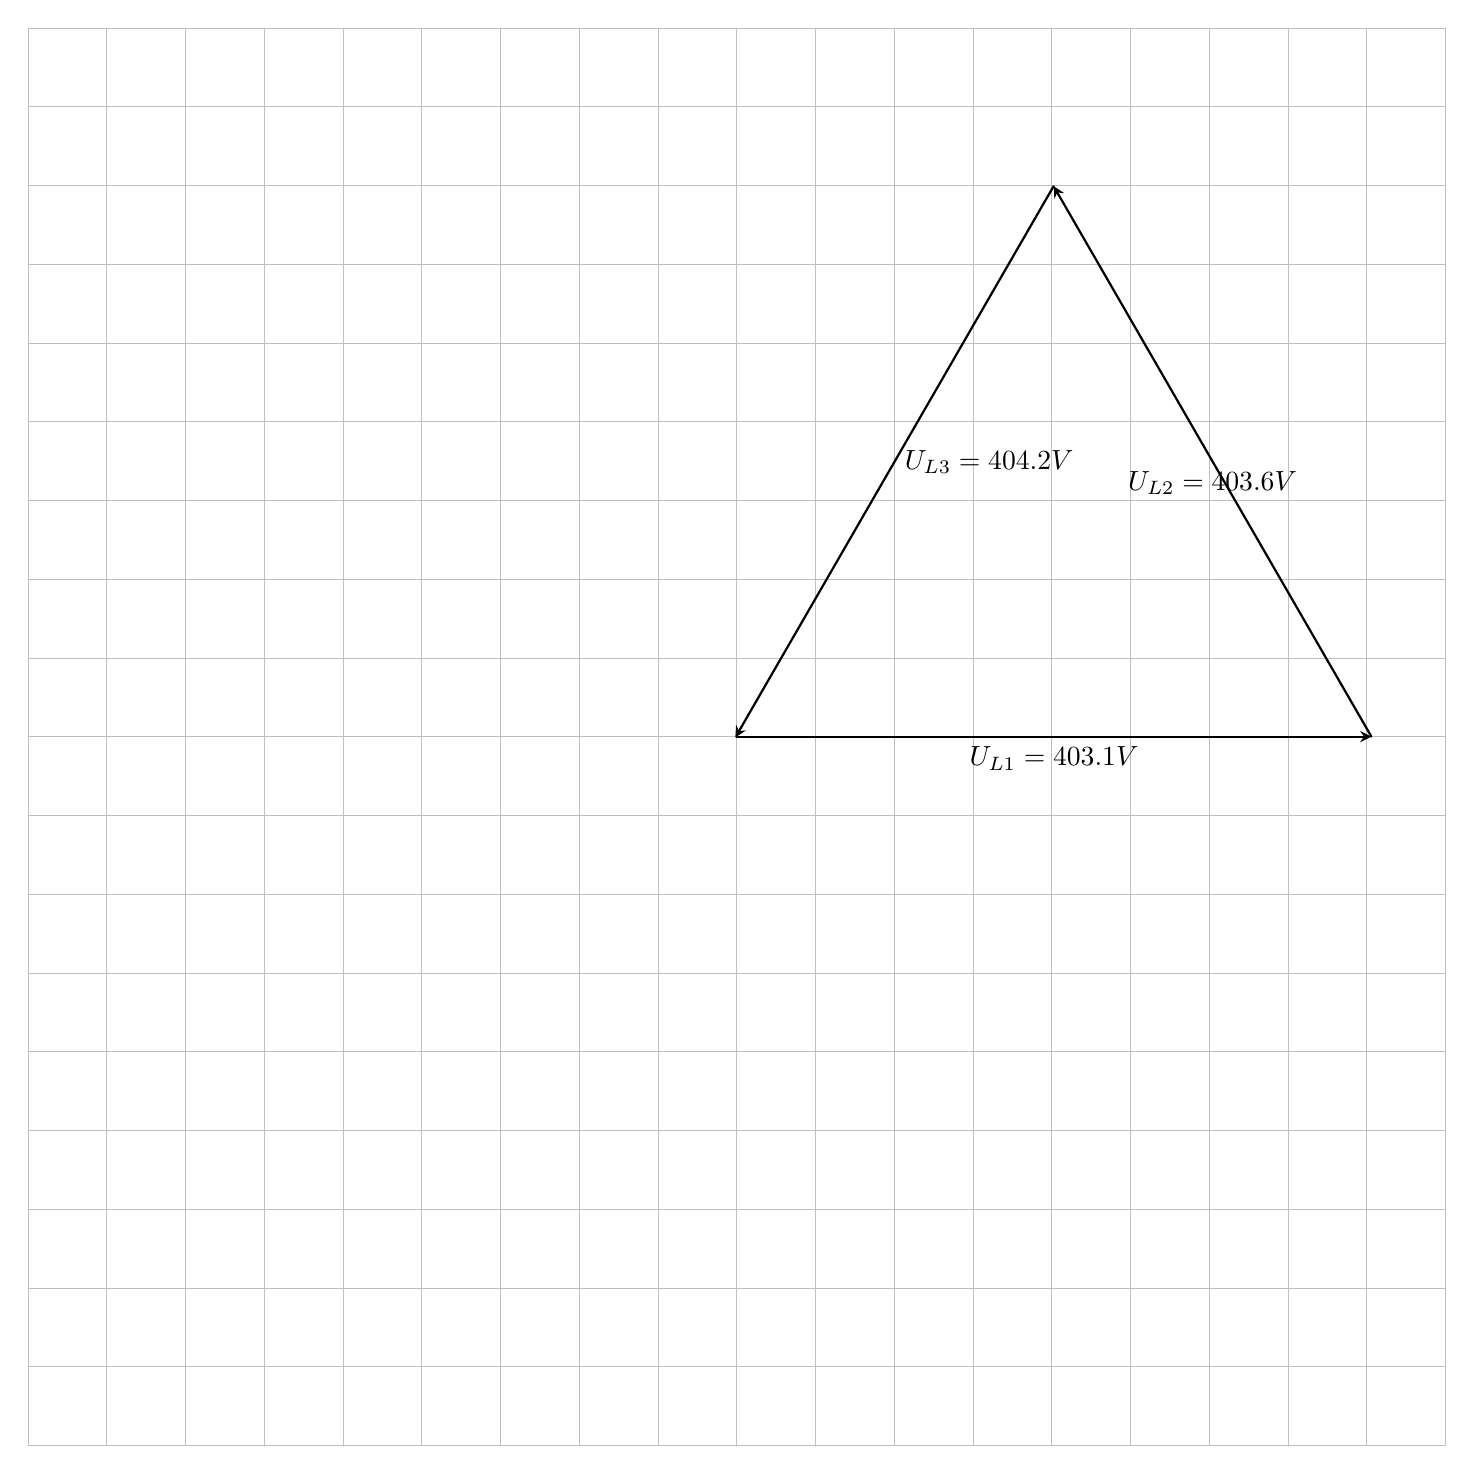
\begin{tikzpicture}[
	>=stealth,
	thick,
	line cap=round,
	line join=round
	]
	\draw[help lines,lightgray] (-9,-9) grid (9,9);
	\begin{scope}[->]
		\draw (0.0,0.0) -- (8.062000000000001,0.0) node[midway,below] {$U_{L1}=403.1V$};
		\draw (8.062000000000001,0.0) -- (4.0260000000000025,6.99055705934799) node[midway,below] {$U_{L2}=403.6V$};
		\draw (4.0260000000000025,6.99055705934799) -- (-0.015999999999995573,-0.010392304845411537) node[midway,right] {$U_{L3}=404.2V$}; 
	\end{scope}
\end{tikzpicture}


% =====================================================
\section{Sym. Dreieck}
% =====================================================
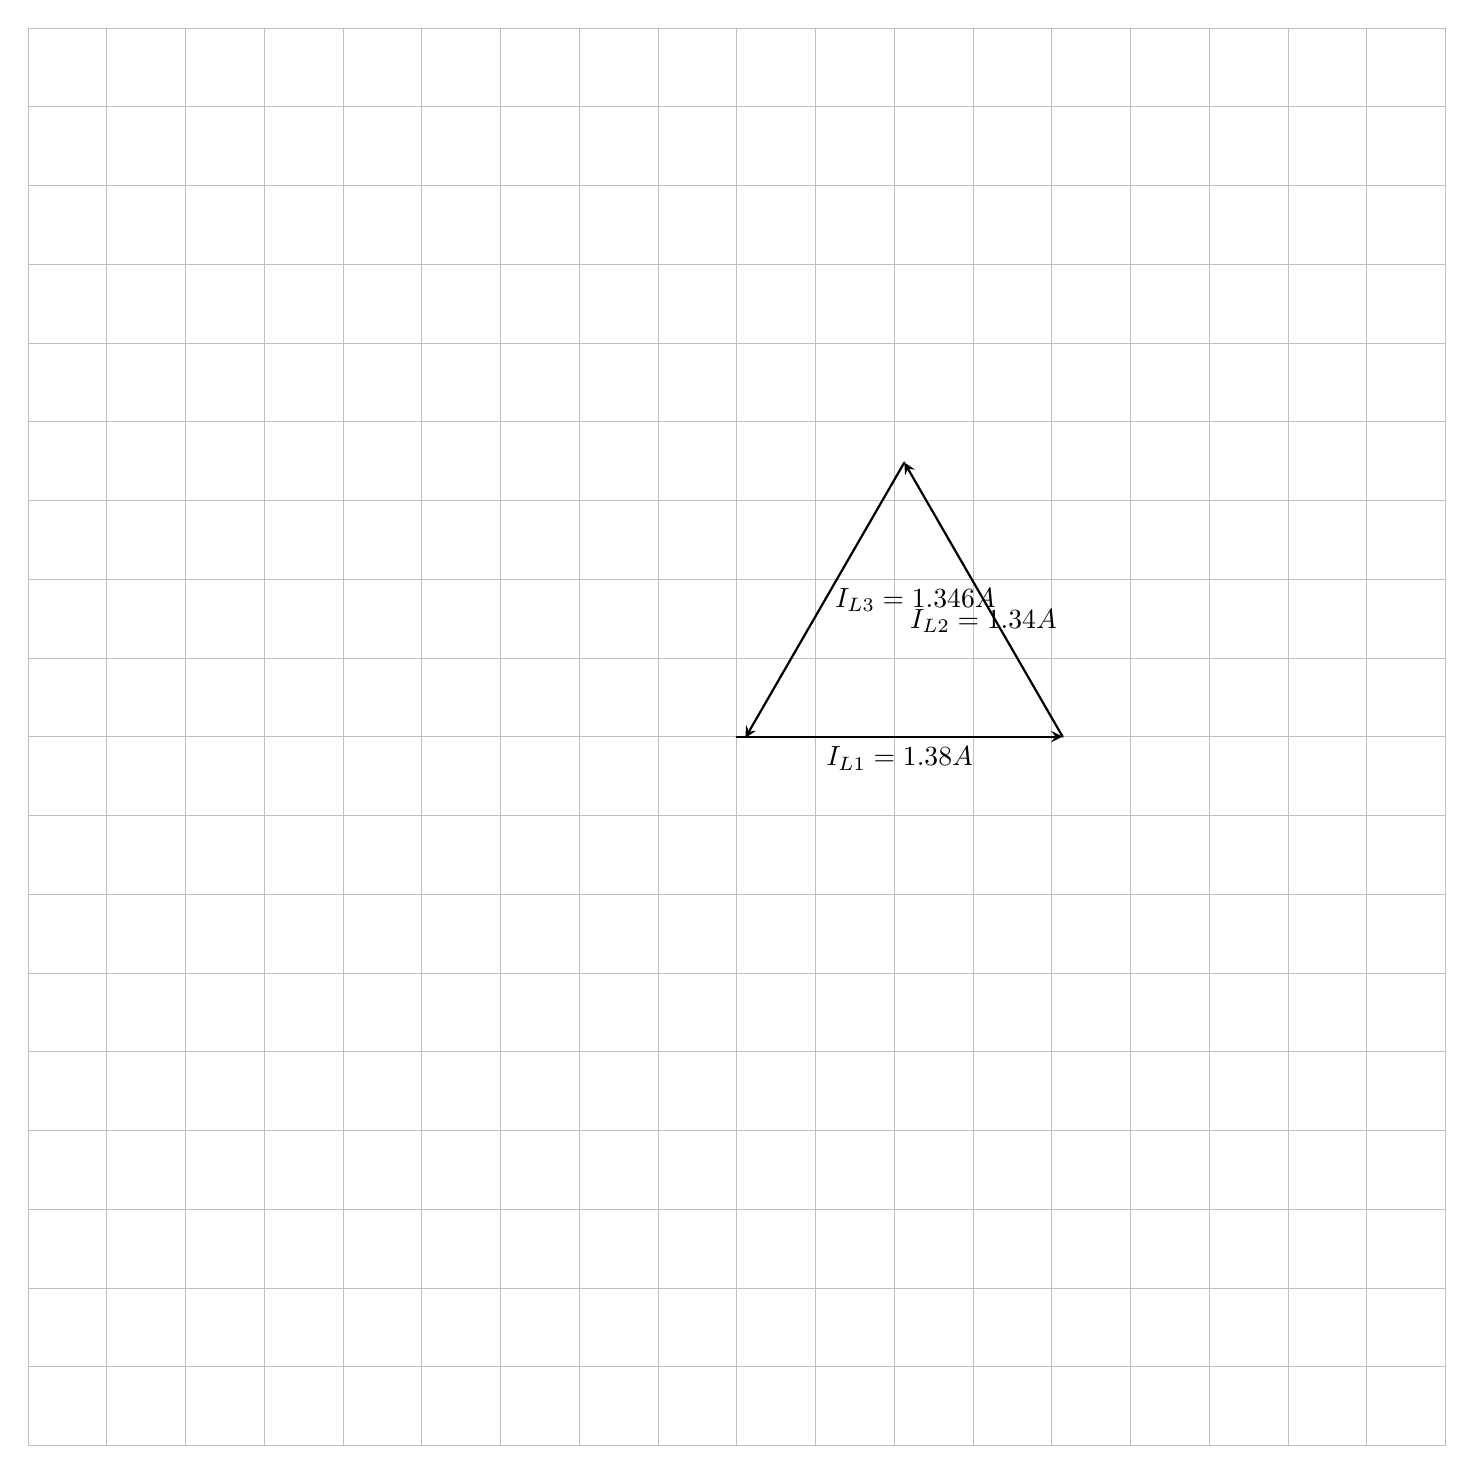
\begin{tikzpicture}[
	>=stealth,
	thick,
	line cap=round,
	line join=round
	]
	\draw[help lines,lightgray] (-9,-9) grid (9,9);
	\begin{scope}[->]
		\draw (0.0,0.0) -- (4.14,0.0) node[midway,below] {$I_{L1}=1.38A$};
		\draw (4.14,0.0) -- (2.1300000000000003,3.481422123213444) node[midway,below] {$I_{L2}=1.34A$};
		\draw (2.1300000000000003,3.481422123213444) -- (0.1110000000000011,-0.015588457268119527) node[midway,right] {$I_{L3}=1.346A$}; 
	\end{scope}
\end{tikzpicture}


% =====================================================
\section{Unsym. Dreieck}
% =====================================================
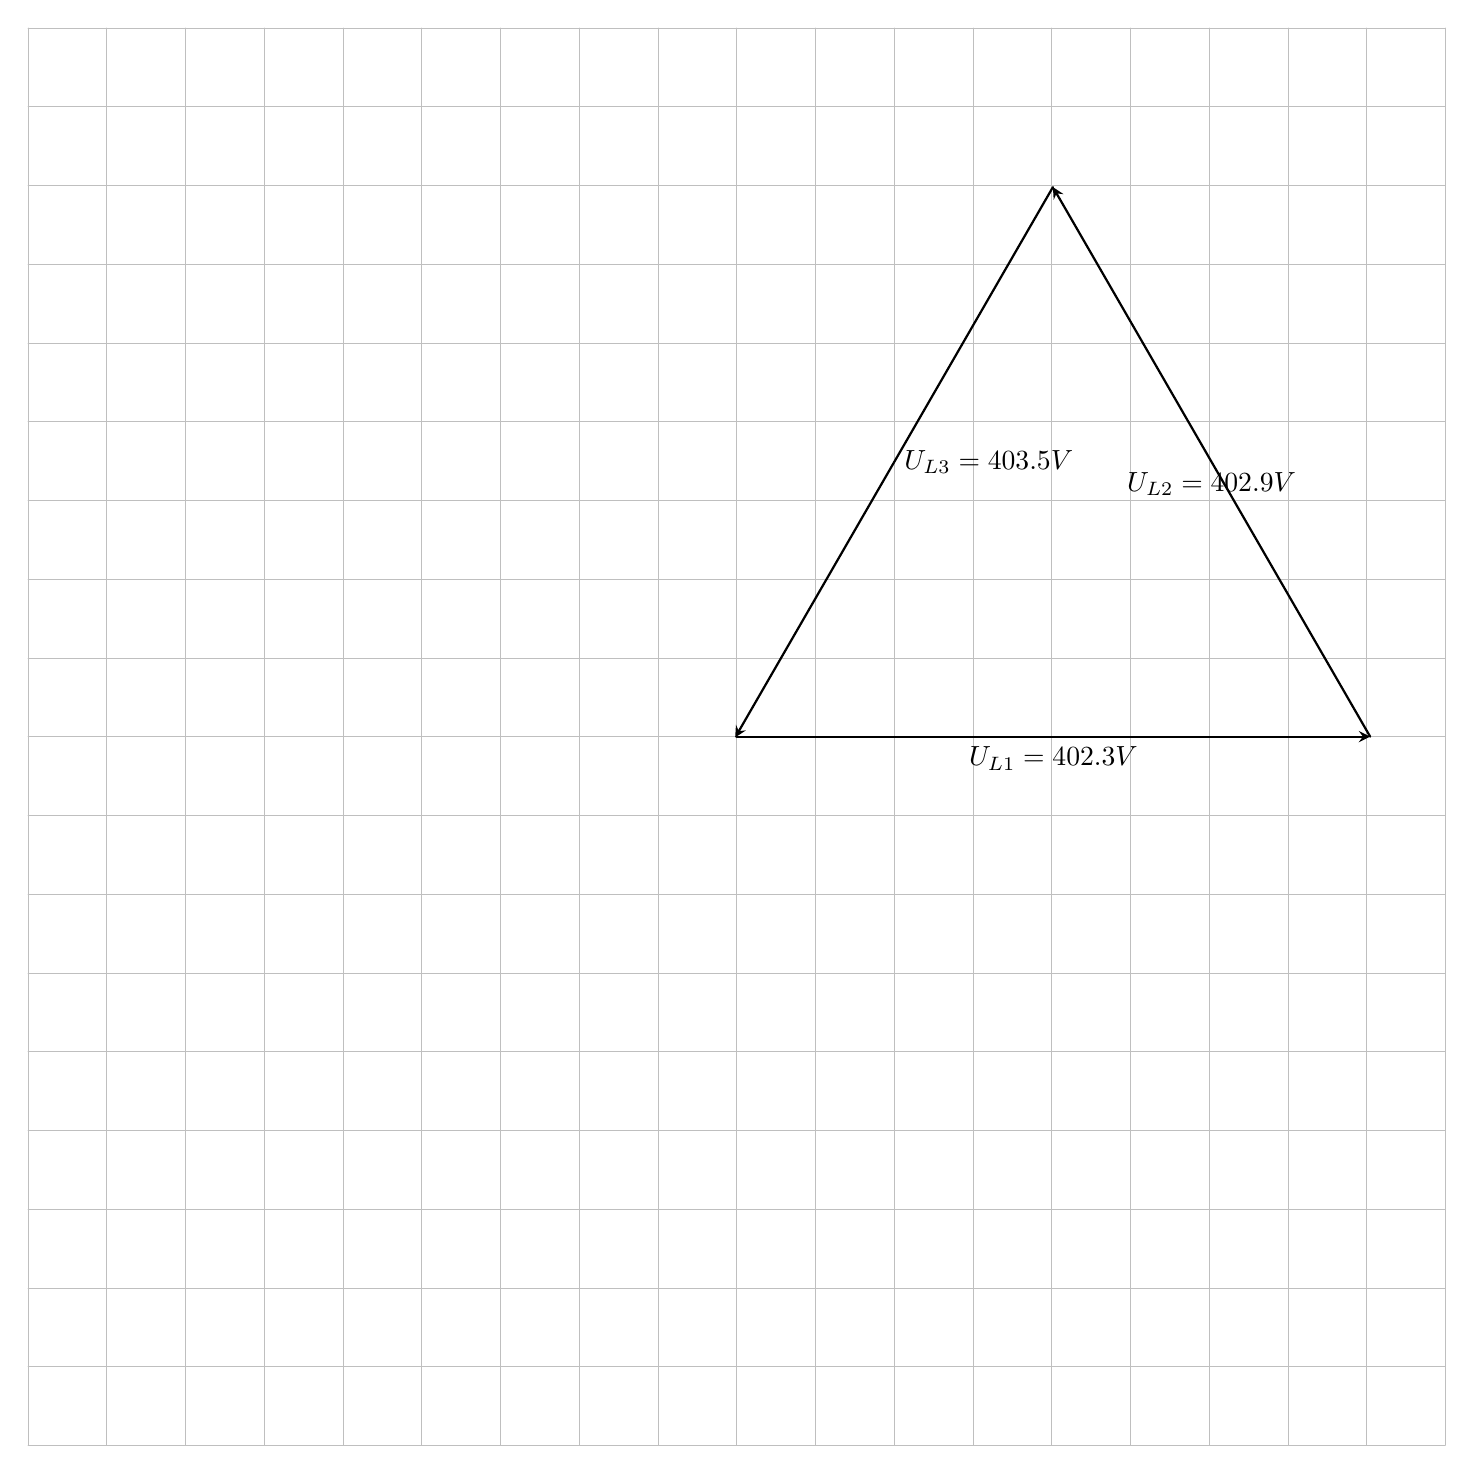
\begin{tikzpicture}[
	>=stealth,
	thick,
	line cap=round,
	line join=round
	]
	\draw[help lines,lightgray] (-9,-9) grid (9,9);
	\begin{scope}[->]
		\draw (0.0,0.0) -- (8.046000000000001,0.0) node[midway,below] {$U_{L1}=402.3V$};
		\draw (8.046000000000001,0.0) -- (4.017000000000003,6.978432703695007) node[midway,below] {$U_{L2}=402.9V$};
		\draw (4.017000000000003,6.978432703695007) -- (-0.017999999999995353,-0.010392304845413314) node[midway,right] {$U_{L3}=403.5V$}; 
	\end{scope}
\end{tikzpicture}


% =====================================================
\section{Unsym. Dreieck}
% =====================================================
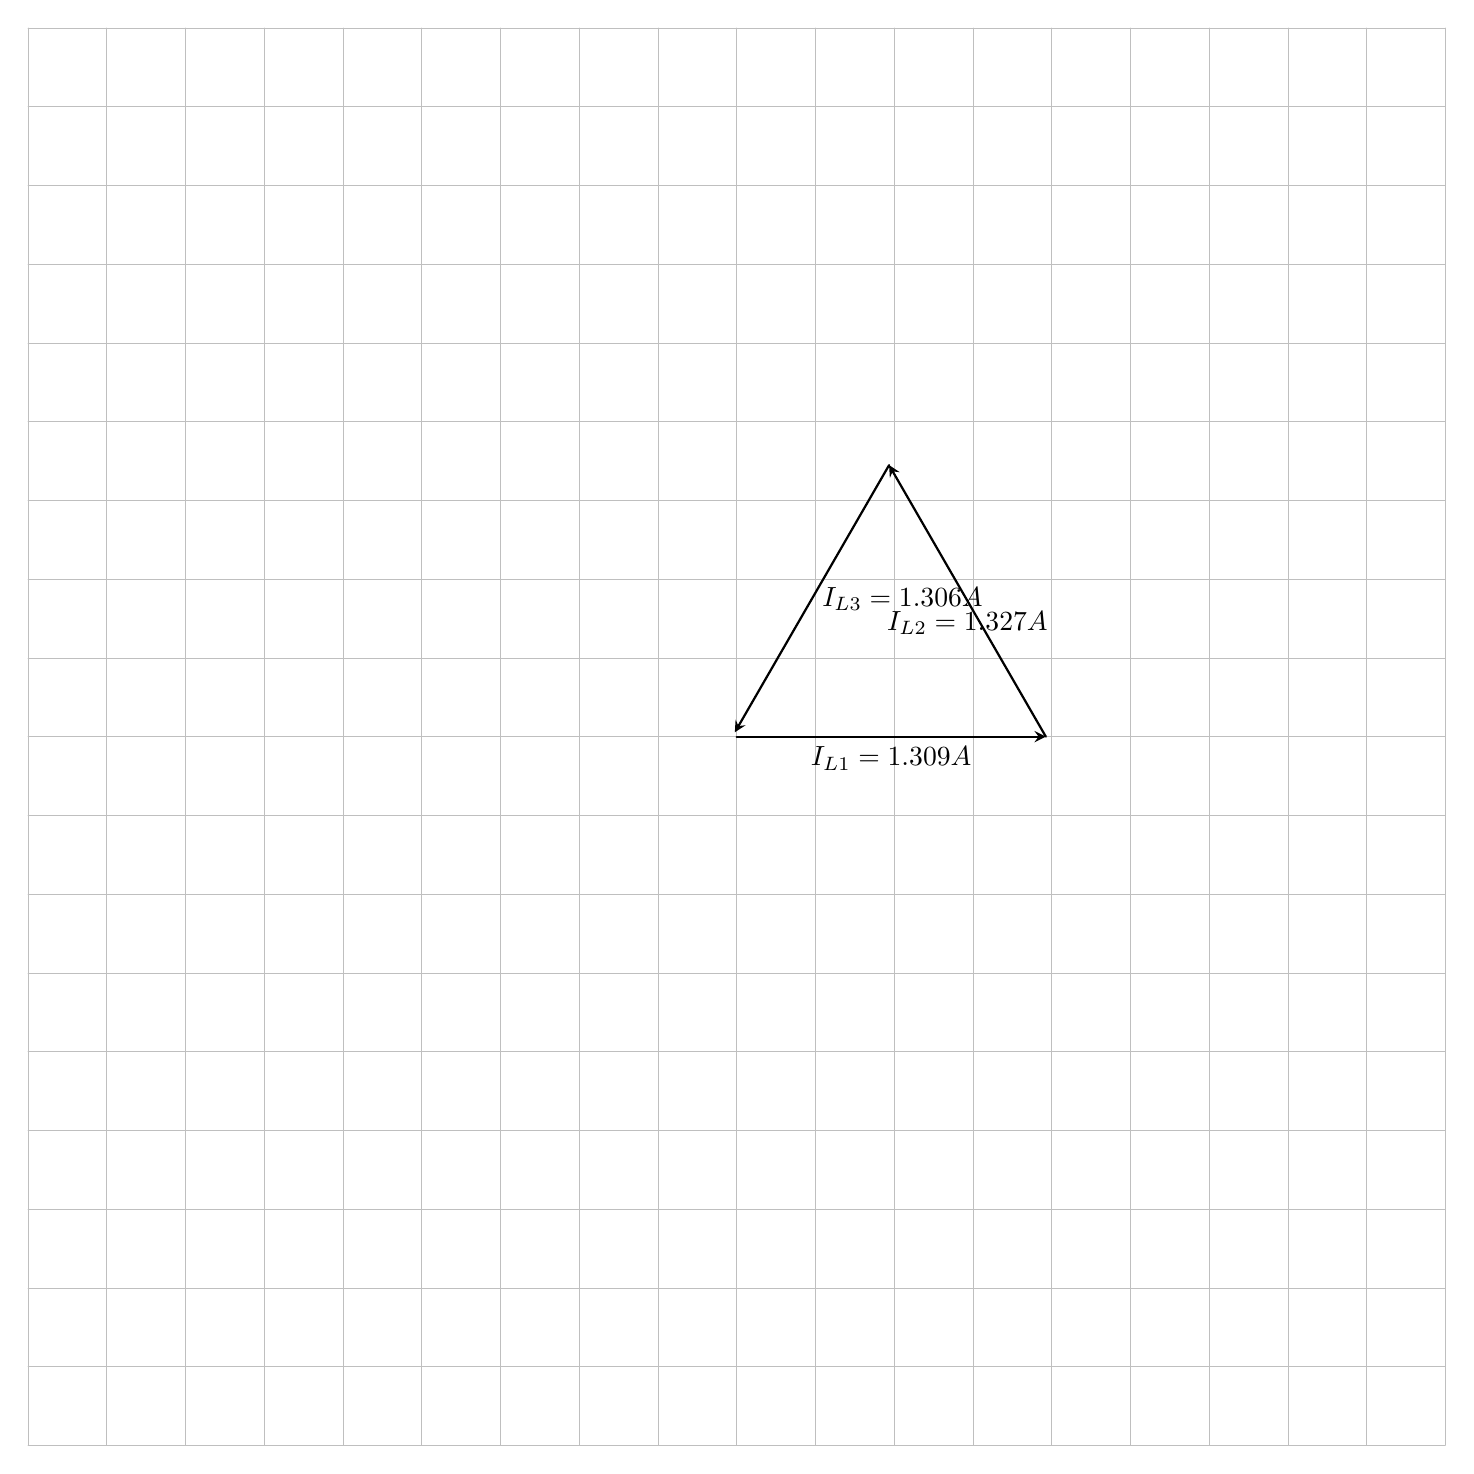
\begin{tikzpicture}[
	>=stealth,
	thick,
	line cap=round,
	line join=round
	]
	\draw[help lines,lightgray] (-9,-9) grid (9,9);
	\begin{scope}[->]
		\draw (0.0,0.0) -- (3.9269999999999996,0.0) node[midway,below] {$I_{L1}=1.309A$};
		\draw (3.9269999999999996,0.0) -- (1.9365000000000006,3.44764713246585) node[midway,below] {$I_{L2}=1.327A$};
		\draw (1.9365000000000006,3.44764713246585) -- (-0.022499999999998632,0.05455960043841923) node[midway,right] {$I_{L3}=1.306A$}; 
	\end{scope}
\end{tikzpicture}


% =====================================================
\section{Unsym. Dreieck}
% =====================================================
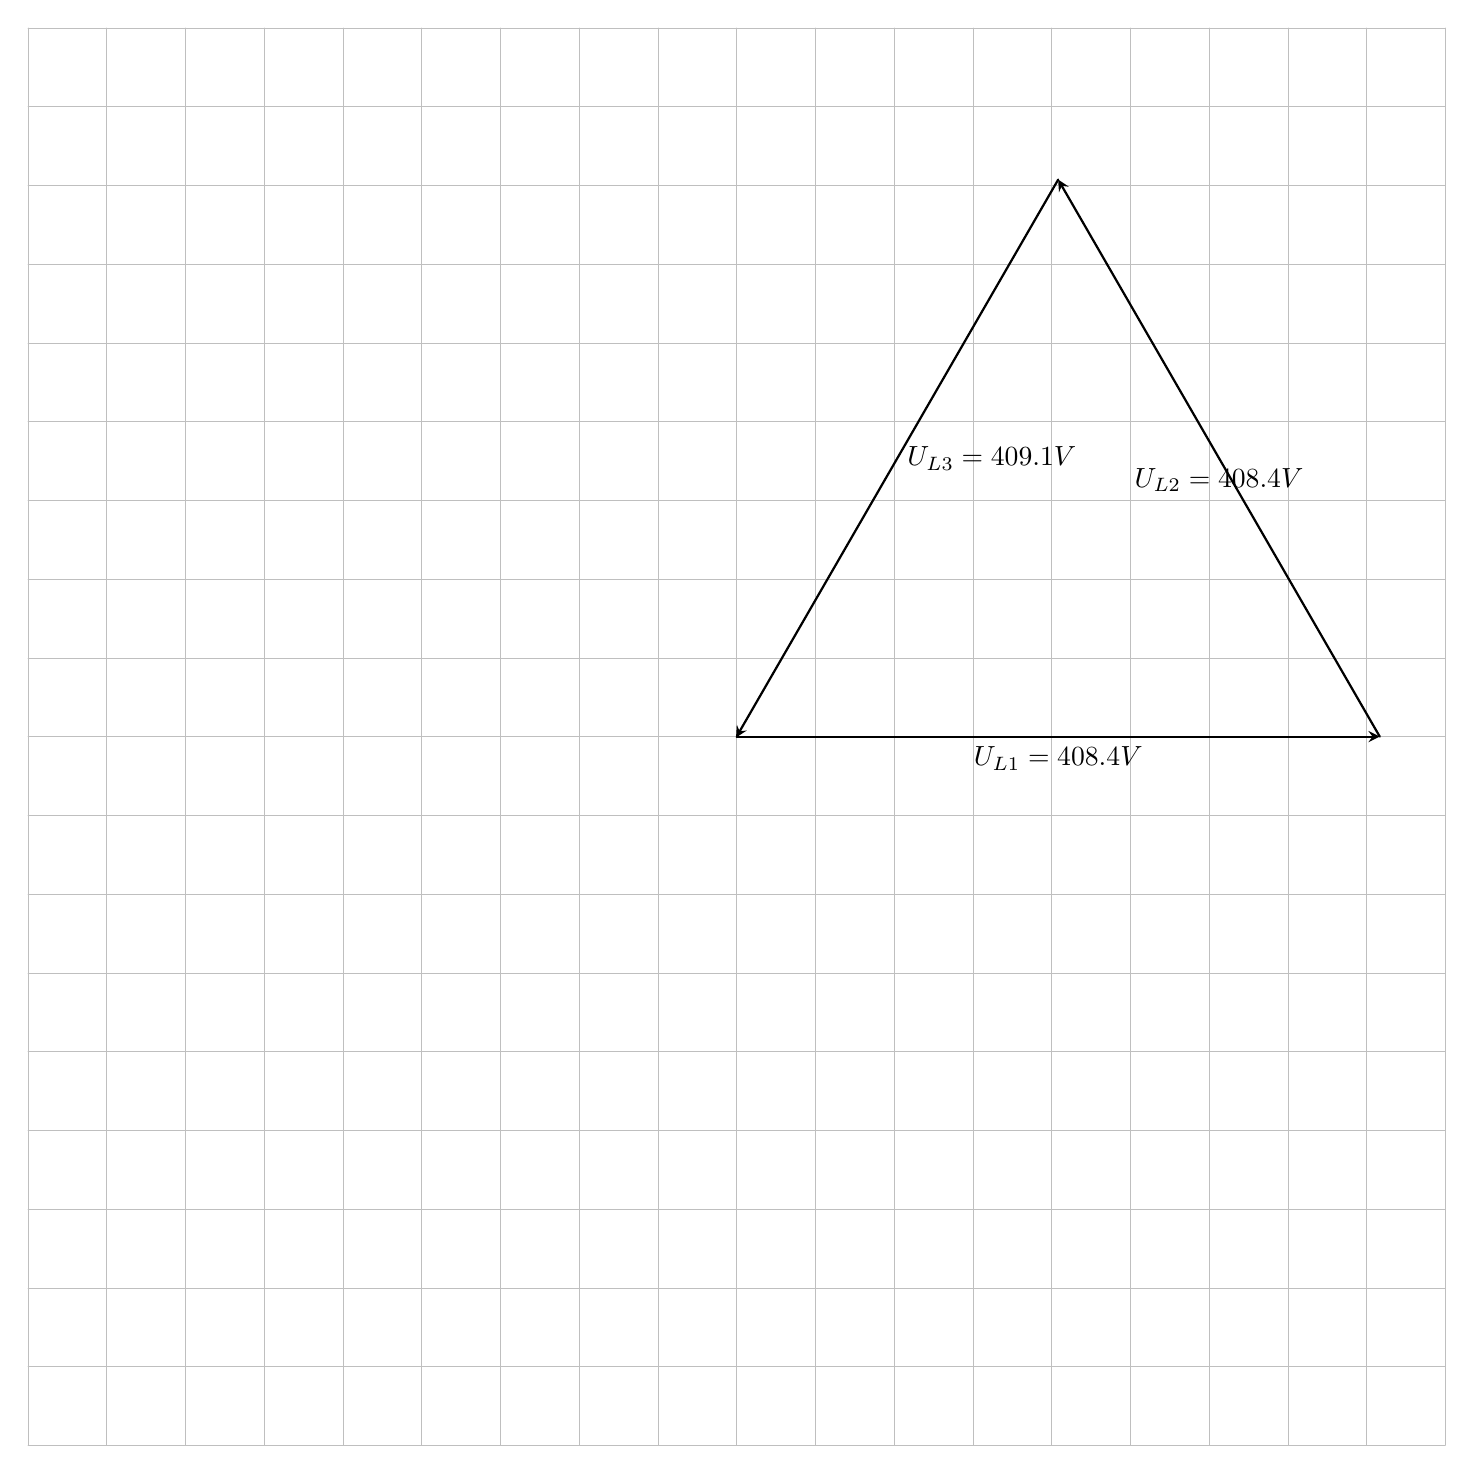
\begin{tikzpicture}[
	>=stealth,
	thick,
	line cap=round,
	line join=round
	]
	\draw[help lines,lightgray] (-9,-9) grid (9,9);
	\begin{scope}[->]
		\draw (0.0,0.0) -- (8.168,0.0) node[midway,below] {$U_{L1}=408.4V$};
		\draw (8.168,0.0) -- (4.084000000000001,7.073695498111295) node[midway,below] {$U_{L2}=408.4V$};
		\draw (4.084000000000001,7.073695498111295) -- (-0.006999999999997009,-0.012124355652982644) node[midway,right] {$U_{L3}=409.1V$}; 
	\end{scope}
\end{tikzpicture}


% =====================================================
\section{Unsym. Dreieck}
% =====================================================
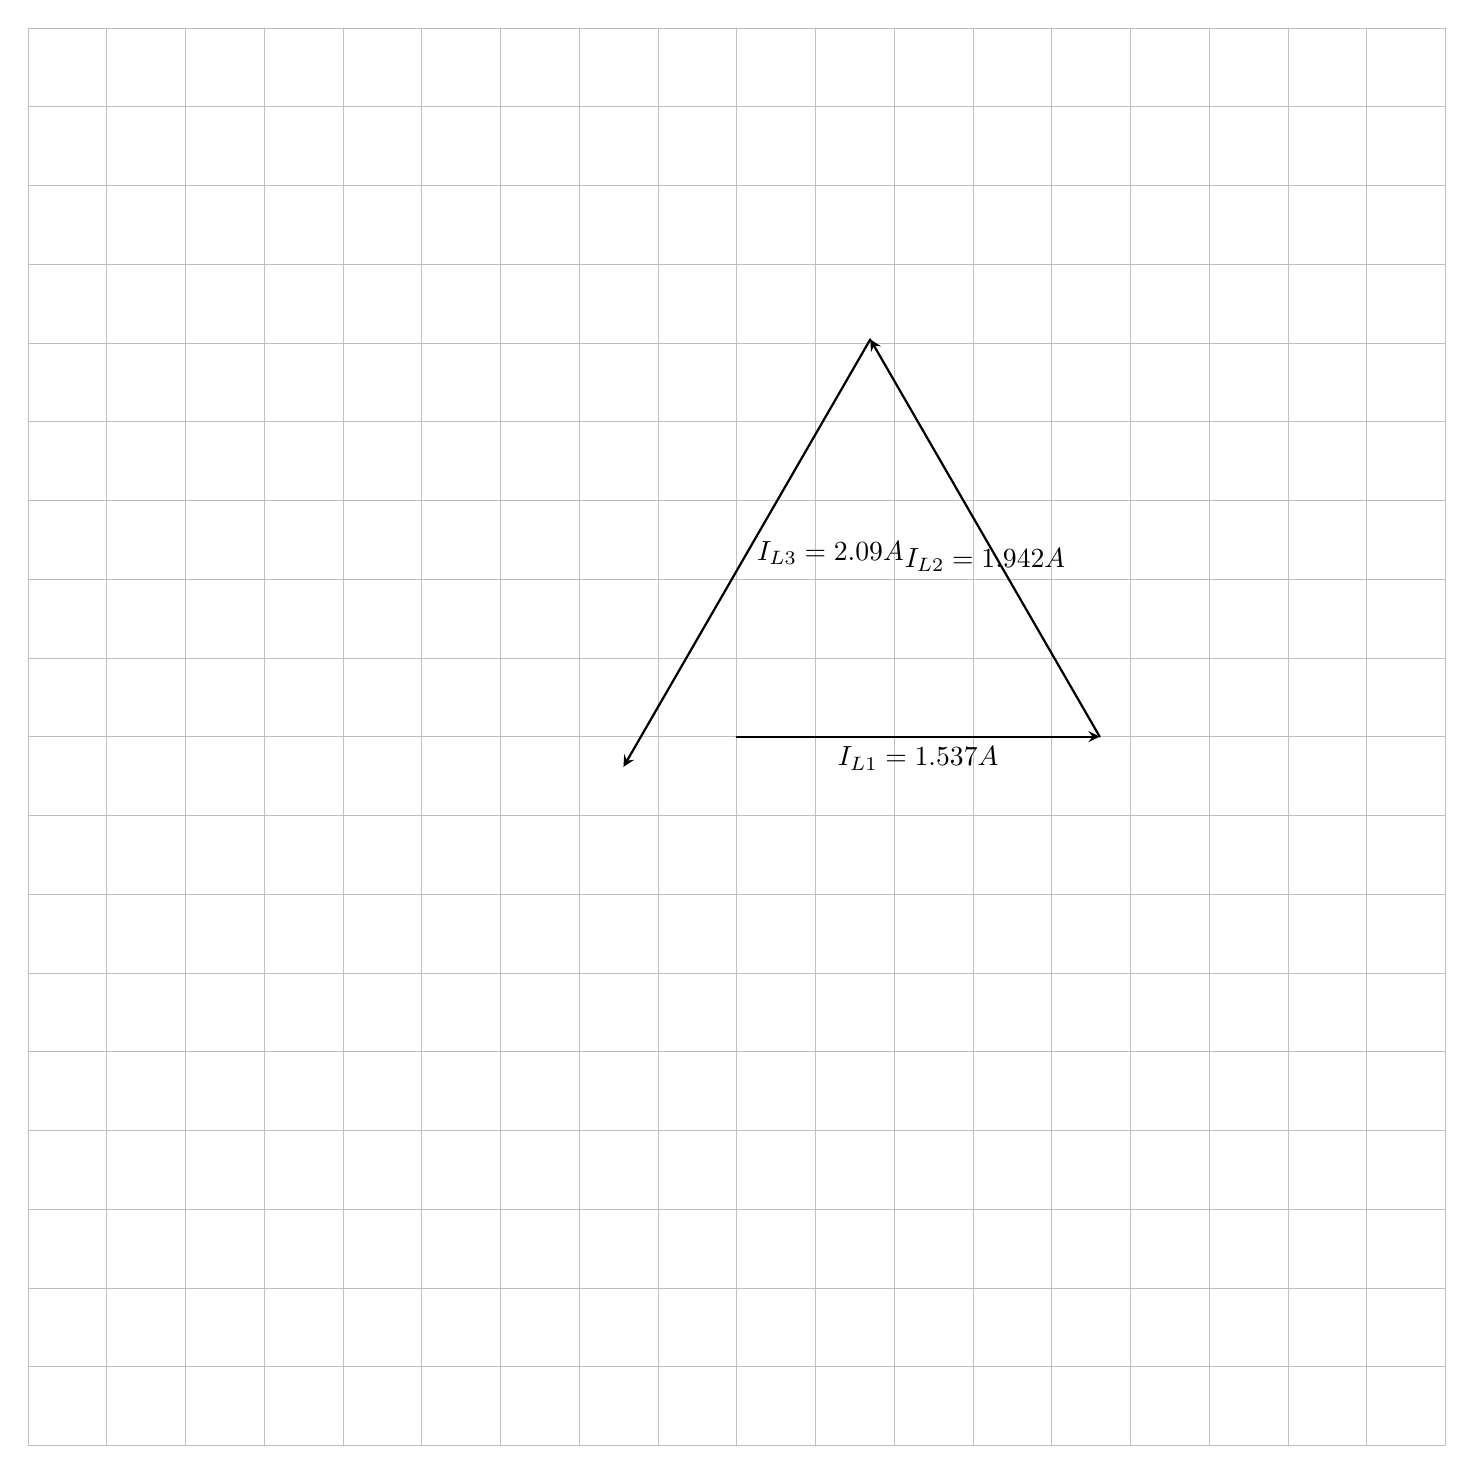
\begin{tikzpicture}[
	>=stealth,
	thick,
	line cap=round,
	line join=round
	]
	\draw[help lines,lightgray] (-9,-9) grid (9,9);
	\begin{scope}[->]
		\draw (0.0,0.0) -- (4.611,0.0) node[midway,below] {$I_{L1}=1.537A$};
		\draw (4.611,0.0) -- (1.6980000000000013,5.045464002448139) node[midway,below] {$I_{L2}=1.942A$};
		\draw (1.6980000000000013,5.045464002448139) -- (-1.4369999999999972,-0.38451527928029083) node[midway,right] {$I_{L3}=2.09A$}; 
	\end{scope}
\end{tikzpicture}





\end{document}


